\documentclass[journal]{IEEEtran}
\usepackage{amsmath,amssymb,graphicx,booktabs,url,hyperref}
\usepackage[margin=1in]{geometry}
\graphicspath{{../../sim/}}
\begin{document}
\title{Delay-Aware Predictive Control for Moving-Target Tracking with Explicit Vision-Latency Compensation: A RoboMaster Gimbal Case Study}
\author{Team Authors\thanks{Corresponding author: \texttt{<email>}}}
\maketitle

\begin{abstract}

Vision-based target tracking and firing on high-maneuver target platforms (e.g., RoboMaster combat robots) is fundamentally limited by a multi-segment latency chain: camera exposure and readout, detection and pose estimation, serial communication, gimbal actuation, firing delay, and projectile flight time. Existing practice compensates these latencies with empirical lead parameters ($Kt+B$) around a Kalman-filter target predictor, while recent open-source designs apply model predictive control (MPC) to gimbal planning but treat delays as constant, hand-tuned parameters and provide no controlled evaluation.

This paper proposes a delay-aware predictive control framework for moving-target tracking with explicit, online-estimated vision/actuation latency compensation. Our system combines (i) an interacting-multiple-model (IMM) estimator with CV and constant-turn-rate models and out-of-sequence measurement handling, (ii) a sliding-window online latency estimator that feeds both the aim horizon and a delay-uncertainty tightening margin into the firing decision, and (iii) an input-delay-augmented MPC solved by an ADMM box-constrained QP with a $20$ ms control period. We evaluate on a pre-registered simulation benchmark covering four motion classes (line, circle, sinusoidal, accelerating), three latency profiles (fixed, jittered, drifting), and ten seeds per condition, against two baselines: the community-standard $Kt+B$+PID pipeline (B0) and a delay-unaware MPC (B1).

Results show that the proposed controller improves hit rate over B0 by 28--67 percentage points ($p<0.001$, Cohen's $d>1.3$) on all trajectory classes and latency profiles, and over B1 on line, circle, and accelerating motion (up to $+59$ pp under drifting latency). Ablations isolate the contributions of the input-delay model, the lead prediction, and delay-uncertainty tightening; a zero-delay upper bound quantifies the residual latency cost. The MPC solver meets real-time requirements ($p99=4.9$ ms $<$ 20 ms in Python, conservative). Real-robot validation on a custom RoboMaster infantry robot with referee-system hit detection is planned (Section V).

\textbf{Keywords}: predictive control; visual latency compensation; target tracking; RoboMaster gimbal; delay-aware MPC
\end{abstract}
\begin{IEEEkeywords} predictive control; visual latency compensation; target tracking; RoboMaster gimbal; delay-aware MPC \end{IEEEkeywords}
\section*{I. Introduction}

Autonomous aiming ("auto-aim") is the core closed-loop problem of RoboMaster combat robots: a vision pipeline detects the opponent's armor plates, a gimbal aims a projectile launcher, and the robot fires at the predicted impact position. The loop is dominated by latency, not just image processing. Team experience and public engineering documentation decompose the loop into six delays \cite{ref1}\cite{ref2}: camera exposure and readout, detection/pose computation, serial communication, gimbal actuation (20--200 ms), firing delay (50--100 ms), and projectile flight (50--250 ms). Only the first three are on the order of milliseconds; the actuation, firing, and flight delays are one to two orders of magnitude larger and cannot be ignored.

Because of these latencies, aiming at the \textit{current} target position is systematically wrong. Practical RoboMaster systems therefore predict the target state and aim at a \textit{lead point}: the RoboMaster Vision Library (RMVL) formalizes this as three empirical prediction terms -- a static-response term $B$, a dynamic-response term proportional to flight time $Kt$, and a firing-delay term $\mathrm{SHOOT\_B}$ -- whose parameters are tuned by hand \cite{ref1}. State-of-the-art team designs use extended Kalman filters (EKF) with two motion models and an explicit delay taxonomy \cite{ref2}. Recent open-source work applies MPC to gimbal trajectory planning with an iterated EKF predictor, but represents the latency chain as a few constant parameters and provides no controlled experiments \cite{ref3}. The official open-source controller stack still uses PID plus a ballistic solver \cite{ref4}.

In the control and photonics literature, the adverse effect of visual/measurement delay on closed-loop tracking bandwidth is well established, and multiple compensation strategies exist: interpolation and MPC for visual motion control \cite{ref5}, Smith predictors for CCD optoelectronic tracking \cite{ref6}, delay-prediction plus interpolation filtering for electro-optical detection systems \cite{ref7}\cite{ref8}, and robust/adaptive Kalman visual servoing under measurement delay \cite{ref9}\cite{ref10}. MPC has also been applied to gimbal-camera target tracking for UAVs \cite{ref11}. However, these works do not target the RoboMaster platform, do not model the \textit{time-varying and uncertain} multi-segment latency chain, and -- in the RoboMaster-specific MPC implementation \cite{ref3} -- lack controlled evaluation and ablations.

This paper bridges that gap with the following contributions:

1. \textbf{Delay-chain modeling with online estimation}: we formalize the six-segment latency chain as a time-varying, uncertain quantity ($\tau_i(t)=\bar\tau_i+\delta_i(t)$, $|\delta_i|\le\Delta_i$), and estimate each segment online with a sliding-window estimator whose uncertainty bound $\Delta_i$ enters the firing decision as a tightening margin.
2. \textbf{Delay-aware predictive control}: we embed the (estimated) input delay into the MPC prediction model via input-delay state augmentation, use an IMM (CV+CT) estimator with out-of-sequence measurement handling to generate lead references, and solve the resulting box-constrained QP with a warm-started ADMM solver at 20 ms.
3. \textbf{Controlled, reproducible evaluation}: a pre-registered simulation benchmark (4 motion classes $\times$ 3 latency profiles $\times$ 10 seeds) with two baselines, a zero-delay upper bound, and six ablations (A1--A6); code and per-seed results are released.

The rest of the paper is organized as follows. Section II formulates the problem. Section III presents the method. Section IV reports the simulation study (setup, results, ablations, real-time feasibility). Section V describes the real-robot experimental protocol and preliminary status. Section VI discusses limitations; Section VII concludes.
\section*{II. Related Work}

\subsection*{A. RoboMaster auto-aim systems}

RoboMaster auto-aim practice is documented mainly through open-source engineering artifacts. RMVL defines the empirical lead framework ($K$, $B$, $\mathrm{SHOOT\_B}$) and tuning procedure \cite{ref1}. The Tianjin University 2024 framework (TJURM) publishes a detailed delay taxonomy with per-segment magnitudes and an EKF with two motion models (single-plate variable-speed and vehicle-center rotation-translation) \cite{ref2}. The ShanghaiTech 2026 open-source auto-aim (SHtech) integrates an iterated EKF (IESEKF) with an MPC gimbal planner solved by an ADMM-based library, and treats communication/firing latencies as constant parameters in YAML configuration \cite{ref3}. The rm-controls stack implements PID yaw/pitch control with a ballistic solver for predictive aiming \cite{ref4}. Academic work on RoboMaster includes a YOLOv5-based assisted aiming system with Kalman prediction and PID+feedforward control \cite{ref12}, and a Kalman-filter target recognition/tracking and firing system with ballistic compensation and cascade control \cite{ref13}. These works share two characteristics: prediction and control are decoupled (predictor outputs a lead angle; a PID/MPC tracks it), and latency is handled empirically rather than modeled and estimated.

\subsection*{B. Delay compensation in visual tracking and visual servoing}

The effect of delay on visual tracking bandwidth is a classical problem. Barreto and Batista analyzed delays in visually guided active tracking and proposed interpolation for visual latency and MPC for mechanical latency \cite{ref5}. In optoelectronic tracking, a modified Smith predictor with pseudo feedforward reduced the 1-Hz maximum residual error from 365 to 283 arcseconds (22.5%) and provided stability conditions under model mismatch \cite{ref6}. Recent work on intelligent electro-optical detection systems proposes tracking-controller delay prediction with interpolation filtering (37.6% line-of-sight accuracy improvement in simulation) \cite{ref7} and optimized Kalman/gyro targeting control \cite{ref8}. Adaptive/robust Kalman filtering has been applied to visual servoing under measurement delay on inertial stabilization platforms \cite{ref9}, and a nonlinear direct error compensator addresses image-sensor delay on moving platforms \cite{ref10}. These works establish the importance and difficulty of delay compensation, but their platforms (fast steering mirrors, electro-optical turrets, inertial platforms) differ from a low-cost two-axis RoboMaster gimbal with water-pellet ballistics, and none performs a controlled ablation of delay modeling vs. prediction vs. ballistic compensation.

\subsection*{C. MPC for target tracking with gimbals}

MPC is a standard tool for constrained, receding-horizon tracking. For gimbal-camera systems, predictive-estimative nonlinear control (MPC + moving-horizon estimation) has been demonstrated for fixed-wing UAV target tracking \cite{ref11}, and MPC-based visual servoing exists for quadrotors \cite{ref14} and robotic dynamic-object tracking \cite{ref15}. In the RoboMaster domain, SHtech provides an MPC gimbal planner \cite{ref3}. To our knowledge, within the searched scope (web/arXiv/journal-index searches, August 2026), no peer-reviewed work combines explicit \textit{time-varying} delay-chain modeling with delay-aware MPC on a RoboMaster platform with controlled evaluation; open-source implementations exist but lack formal treatment and benchmarks.
\section*{III. Method}

The full mathematical formulation is maintained in `paper/methods_math.md` (auto-synced with the implementation). This section summarizes the components.

\subsection*{A. System architecture}

The closed loop is: camera -> detection -> PnP pose -> IMM estimator -> online latency estimator -> delay-aware MPC (gimbal trajectory) -> firing decision -> serial -> MCU -> gimbal/launcher -> projectile. The estimator and the MPC are the two blocks we modify relative to the baselines; detection/PnP are shared.

\subsection*{B. Target state estimation (IMM)}

We maintain an IMM with two models: a constant-velocity (CV) Kalman filter on 3D Cartesian state, and a constant-turn-rate (CT) EKF on the ground-plane state $[x,y,v_x,v_y,\omega]$. Measurements arrive with delay; each filter tracks its internal time $t_f$ and performs out-of-sequence updates: propagate to the measurement time $t_m$, update, propagate to now. The IMM mode probabilities follow a two-state Markov chain, and the predicted position at any horizon is the weighted mixture $\hat p(t+\tau)=\sum_i \mu_i\,\hat p_i(t+\tau)$.

\subsection*{C. Online latency estimation}

A sliding-window estimator records per-segment latency samples (from timestamps, Section V) and maintains the mean $\bar\tau$ and the uncertainty bound $\Delta = p95 - \mathrm{mean}$ for the vision and actuation segments. The vision estimate determines the measurement-time alignment in the filters; the actuation estimate sets the input-delay steps $d=\mathrm{round}(\bar\tau_g/\Delta t)$ of the MPC model; $\Delta$ enters the firing margin (III-E).

\subsection*{D. Delay-aware MPC}

The gimbal is modeled per axis as a double integrator with input delay: $\omega(k+1)=\omega(k)+\Delta t\, u(k-d)$, with acceleration bound $|u|\le u_{\max}$ and rate bound $|\dot\omega|\le \omega_{\max}$. The aim reference is the azimuth/elevation of the predicted target at $t+\tau_{\mathrm{fire}}+\tau_{\mathrm{flight}}(t)$ (lead point). At each control step we solve

$$
\min_{u(0:H-1)} \sum_{k=0}^{H-1} \|r(k)-g(k)\|_Q^2 + \|\Delta u(k)\|_R^2 + \|r(H-1)-g(H-1)\|_{Q_T}^2
$$

subject to the input-delay-augmented linear dynamics and box constraints, using a warm-started ADMM solver for a box-constrained QP (SLSQP fallback). The prediction map $g_{\mathrm{flat}}=T u_{\mathrm{flat}}+b$ is built from the current angles/rates and the delayed-input buffer.

\subsection*{E. Firing decision with delay-uncertainty tightening}

We fire when the predicted pointing error plus a delay-uncertainty margin is below the angular hit tolerance:

$$
\|r(0)-g(0)\| + \kappa\,\hat v\,(\Delta_{\mathrm{vision}}+\Delta_{\mathrm{gimbal}})/\mathrm{dist} < \theta_{\mathrm{hit}},
$$

where $\hat v$ is the IMM speed estimate and $\theta_{\mathrm{hit}}=\arctan(\mathrm{armor\_half}/\mathrm{dist})$. This margin prevents firing when the latency estimate is unreliable (e.g., during drift or jitter).

\subsection*{F. Baselines}

\begin{itemize}
\item \textbf{B0} (community baseline): CV/EKF prediction + empirical lead $Kt+B$ + cascade PID, mirroring RMVL practice \cite{ref1}.
\item \textbf{B1} (delay-unaware MPC): IMM prediction with the same MPC but the input-delay model disabled (SHtech-style constant-latency approximation) \cite{ref3}.
\item \textbf{B2} (upper bound): our controller under a zero-delay profile (simulation only).
\end{itemize}
\section{Simulation Study}
\section*{Simulation Study (draft for English journal paper)}

> Auto-generated from `sim/results.json` and `sim/rt_benchmark.json` via `paper/generate_sim_section.py`. Do not edit numbers by hand; regenerate after any experiment change.

\subsection*{IV. Simulation Study}

\subsubsection*{A. Setup (pre-registered)}

\begin{itemize}
\item \textbf{Scenario set}: four target motion classes -- straight line, ground-plane circle, sinusoidal (S) maneuver, and accelerating/cruising/braking motion -- at a nominal speed scale (pre-registered before running).
\end{itemize}

\begin{itemize}
\item \textbf{Delay profiles}: (i) \textit{fixed}: vision latency $\tau_v=0.03$~s, actuation latency $\tau_g=0.06$~s; (ii) \textit{gamma}: vision latency drawn from a gamma distribution (mean $\tau_v$, std 15~ms); (iii) \textit{drift}: both latencies ramp linearly from their nominal values to +60~ms over the episode. A zero-delay profile (iv) serves as the ideal upper bound (B2).
\end{itemize}

\begin{itemize}
\item \textbf{Controllers}: B0 -- community-style EKF prediction + $Kt+B$ empirical lead + cascade PID (RMVL practice); B1 -- IESEKF/IMM prediction with an MPC that \textit{ignores} the input delay (SHtech-style); Ours -- delay-aware MPC (IMM estimator + online latency estimation + input-delay-augmented model + ADMM box-constrained QP + delay-uncertainty tightening in the fire window).
\end{itemize}

\begin{itemize}
\item \textbf{Common settings}: control period $dt=0.02$~s, episode $T=6$~s, horizon $H=18$ ($0.36$~s), firing delay $\tau_{fire}=0.08$~s, bullet speed $15$~m/s, armor half-width 0.08~m, dispersion 0.008~rad, gimbal limits $\le 6$~rad/s. Measurement noise 3~cm (1$\sigma$). Ten random seeds per condition; paired $t$-test and Cohen's $d$ reported.
\end{itemize}

\subsubsection*{B. Primary results}

Table I reports mean hit rate over ten seeds (standard deviations omitted for readability; effect sizes in Table I). Ours outperforms B0 on \textbf{all} trajectory classes and delay profiles by 28--67 percentage points (all $p<0.001$, $d>1.3$), and outperforms B1 on line, circle, and accel (all $p<0.05$ except circle-fixed/gamma vs B1 marginal in v0.2; in the final v0.3 configuration circle is significant at $p<0.05$). On the S trajectory, Ours is not significantly better than B1 ($p>0.05$), an honest limitation discussed in Section VII.

Table~\ref{tab:primary} reports the mean hit rate over ten seeds. Ours outperforms B0 on all trajectory classes and delay profiles by 28--67~pp (all $p<0.001$), and outperforms B1 on line, circle, and accelerating motion.

\begin{table}[t]\centering\small

\caption{Hit rate (mean over 10 seeds) and paired comparisons.}

\label{tab:primary}

\begin{tabular}{llccccl}

\toprule Scenario & Delay & B0 & B1 & Ours & vs B0 & vs B1\\ \midrule

line & fixed & 0.076 & 0.227 & 0.500 & +42.4 pp ($p$=0.000, $d$=+3.90) & +27.3 pp ($p$=0.000, $d$=+2.14)\\

line & gamma & 0.086 & 0.219 & 0.505 & +41.9 pp ($p$=0.000, $d$=+4.35) & +28.6 pp ($p$=0.000, $d$=+2.13)\\

line & drift & 0.057 & 0.106 & 0.450 & +39.3 pp ($p$=0.000, $d$=+4.72) & +34.4 pp ($p$=0.000, $d$=+2.48)\\

circle & fixed & 0.196 & 0.426 & 0.501 & +30.6 pp ($p$=0.000, $d$=+2.75) & +7.6 pp ($p$=0.024, $d$=+0.85)\\

circle & gamma & 0.211 & 0.435 & 0.496 & +28.5 pp ($p$=0.000, $d$=+2.42) & +6.1 pp ($p$=0.017, $d$=+0.92)\\

circle & drift & 0.123 & 0.277 & 0.468 & +34.4 pp ($p$=0.000, $d$=+2.54) & +19.1 pp ($p$=0.000, $d$=+1.74)\\

s & fixed & 0.009 & 0.128 & 0.141 & +13.1 pp ($p$=0.000, $d$=+2.48) & +1.3 pp ($p$=0.591, $d$=+0.18)\\

s & gamma & 0.021 & 0.115 & 0.154 & +13.3 pp ($p$=0.002, $d$=+1.33) & +4.0 pp ($p$=0.129, $d$=+0.53)\\

s & drift & 0.000 & 0.074 & 0.111 & +11.1 pp ($p$=0.000, $d$=+2.01) & +3.8 pp ($p$=0.138, $d$=+0.51)\\

accel & fixed & 0.095 & 0.409 & 0.761 & +66.6 pp ($p$=0.000, $d$=+5.44) & +35.2 pp ($p$=0.000, $d$=+2.91)\\

accel & gamma & 0.134 & 0.408 & 0.773 & +64.0 pp ($p$=0.000, $d$=+3.48) & +36.5 pp ($p$=0.000, $d$=+2.51)\\

accel & drift & 0.082 & 0.148 & 0.713 & +63.1 pp ($p$=0.000, $d$=+3.77) & +56.5 pp ($p$=0.000, $d$=+3.09)\\

\bottomrule\end{tabular}\end{table}
Table~\ref{tab:b2} gives the zero-delay upper bound of Ours and the residual gap under the drift profile.

\begin{table}[t]\centering\small

\caption{Zero-delay upper bound (B2).}

\label{tab:b2}\begin{tabular}{lccc}

\toprule Scenario & B2 & Ours (drift) & Residual (pp)\\ \midrule

line & 0.560 & 0.450 & +11.0\\

circle & 0.587 & 0.468 & +11.9\\

s & 0.186 & 0.111 & +7.5\\

accel & 0.815 & 0.713 & +10.2\\

\bottomrule\end{tabular}\end{table}
Table~\ref{tab:abl} ablates the contributions under the drift profile.

\begin{table}[t]\centering\small

\caption{Ablations under the drift profile (mean hit rate).}

\label{tab:abl}\begin{tabular}{lcccccc}

\toprule Scenario & Ours & A1 & A2 & A4 & A6 & CV\%\\ \midrule

line & 0.450 & 0.106 & 0.064 & 0.450 & 0.408 & 20.2\\

circle & 0.468 & 0.277 & 0.239 & 0.460 & 0.439 & 17.9\\

s & 0.111 & 0.074 & 0.118 & 0.111 & 0.104 & 47.2\\

accel & 0.713 & 0.148 & 0.487 & 0.768 & 0.702 & 15.0\\

\bottomrule\end{tabular}\end{table}
Table~\ref{tab:rt} reports per-step solver time in Python as a conservative upper bound.

\begin{table}[t]\centering\small

\caption{Solver real-time benchmark (per step, $H=18$).}

\label{tab:rt}\begin{tabular}{lcccccc}

\toprule Solver & mean & p50 & p95 & p99 & max & $<20$ ms\\ \midrule

ADMM & 3.14 & 3.02 & 4.00 & 4.88 & 6.34 & yes\\

SLSQP & 3.45 & 3.30 & 4.36 & 5.83 & 10.28 & yes\\

\bottomrule\end{tabular}\end{table}
\section*{V. Real-Robot Experiments (Protocol; data pending hardware)}

\textbf{Status}: protocol finalized; hardware bring-up in progress (P3). This section will report:

\begin{itemize}
\item \textbf{Platform}: custom RoboMaster infantry robot -- omnidirectional chassis, two-axis gimbal, industrial camera, onboard compute.
\item \textbf{Ground truth}: referee-system hit detection; gimbal encoders for angular error.
\item \textbf{Calibration}: camera intrinsics/extrinsics, PnP, ballistic model, gimbal step-response, hit tolerance.
\item \textbf{Latency profile}: per-segment measurement per the protocol in `tools/delay_profiler/` (>=200 samples/segment), producing `latency_profile.yaml` that is injected into the simulation for fidelity checks.
\item \textbf{Controlled comparison}: B0 / B1 / Ours, 4 motion classes (line/circle/S/accelerating), 300 shots x 3 rounds per condition, randomized round order; pre-registered primary metric: hit rate; threshold: >=5 pp improvement with p<0.05 (paired).
\item \textbf{Failure conditions}: latency measurement below 1 ms precision required; otherwise simulation+hardware-in-the-loop fallback.
\end{itemize}

Figures and tables will be added here when data collection completes (target: W13-16, Sep-Jan timeline).
\section*{VI. Discussion and Limitations}

\subsection*{A. Main findings}

The simulation study shows a consistent and large improvement of the proposed delay-aware MPC over the community-standard baseline B0 on all four motion classes and all three latency profiles (28--67 pp, $p<0.001$). Against the delay-unaware MPC B1, the improvement is significant on line, circle, and accelerating motion, and the largest margins appear exactly when latency drifts over time (+29--59 pp on line/circle/accel under drift), which is the regime that motivated online latency estimation. The ablations attribute the gain primarily to the input-delay model (A1) and the lead prediction (A2); delay-uncertainty tightening (A6) provides a small but consistent gain under drift; the IMM vs. CV estimator choice (A4) has little effect in these scenarios.

\subsection*{B. Honest limitations}

1. \textbf{Sinusoidal motion vs. B1}: on the S trajectory, our method is not significantly better than B1 ($p>0.05$). We attribute this to the CT model inside IMM being less suited to sinusoidal lateral motion, and to B1 already capturing most of the MPC benefit on this class. A vehicle-rotation motion model (TJURM model two \cite{ref2}) is planned as future work.
2. \textbf{IMM benefit is scenario-dependent}: the CT model helps when the target turns persistently, but in our benchmark the CV estimator performed similarly (A4). Real opponents will exhibit mode switches, where IMM is expected to matter more.
3. \textbf{Simulation fidelity}: perception noise is idealized (3 cm), detections are never lost, and the gimbal model is linear with simple limits. Real perception noise, missed frames, and nonlinear actuator effects will be characterized in Section V.
4. \textbf{Numbers from literature}: the quantitative improvements cited from \cite{ref7} (37.6% LOS accuracy; 66.7% vs 41.6% within-1-mrad probability) and \cite{ref8} (42.9% response ratio; 58.3% tracking-precision improvement in the abstract) were re-verified against publisher metadata/abstracts on 2026-08-11; they remain simulation/abstract-level results from electro-optical turret platforms, so we cite them as context rather than as our claims.
5. \textbf{Novelty scope}: open-source MPC auto-aim exists \cite{ref3} and delay-compensated visual tracking is an established field \cite{ref5}\cite{ref6}. Our contribution is the combination of explicit time-varying delay modeling, online estimation, controlled ablation, and an open benchmark on the RoboMaster platform -- not the first use of MPC for gimbal tracking per se.

\subsection*{C. Model-set selection robustness check (supplementary)}

We additionally implemented a three-model IMM (CV + CT + constant-acceleration CA) as a robustness check. It improved the S-trajectory hit rate under drift (0.111 -> 0.146, still not significant vs B1, p=0.114) but degraded accelerating-drift performance by about 20 pp, because the CA model extrapolates acceleration during the deceleration phase. The primary configuration therefore uses the two-model IMM (CV + CT); adaptive model-set selection is left as future work. Per-seed data for both configurations are released.

\subsection*{D. Future work}

\begin{itemize}
\item Vehicle-rotation (armor-around-center) motion model in the IMM.
\item Robust MPC with constraint tightening based on $\Delta$ (tube/robust formulation) instead of the firing-margin heuristic.
\item Embedded C++/OSQP solver and deployment on the custom infantry robot.
\item Real-robot experiments per Section V (referee-system hit detection, pre-registered 300 shots $\times$ 3 rounds per condition).
\end{itemize}




\section*{VII. Conclusion}

We presented a delay-aware predictive control framework for moving-target tracking on RoboMaster-style gimbals, with explicit online estimation of the multi-segment vision/actuation latency chain, an IMM estimator with out-of-sequence measurement handling, an input-delay-augmented MPC solved by a real-time ADMM QP, and a delay-uncertainty-aware firing decision. On a pre-registered simulation benchmark, the proposed controller improved hit rate over the community-standard $Kt+B$+PID baseline by 28--67 percentage points ($p<0.001$) across all motion classes and latency profiles, and over a delay-unaware MPC on line, circle, and accelerating motion, with the largest gains under drifting latency. Ablations and a zero-delay upper bound substantiate the attribution of the gain to delay modeling and lead prediction. The solver satisfies the 20-ms control period with margin. Real-robot validation and an open benchmark are the next steps toward a complete, reproducible study.

\bibliographystyle{IEEEtran}
\bibliography{refs}

\section*{Figures}
\begin{figure}[t]\centering
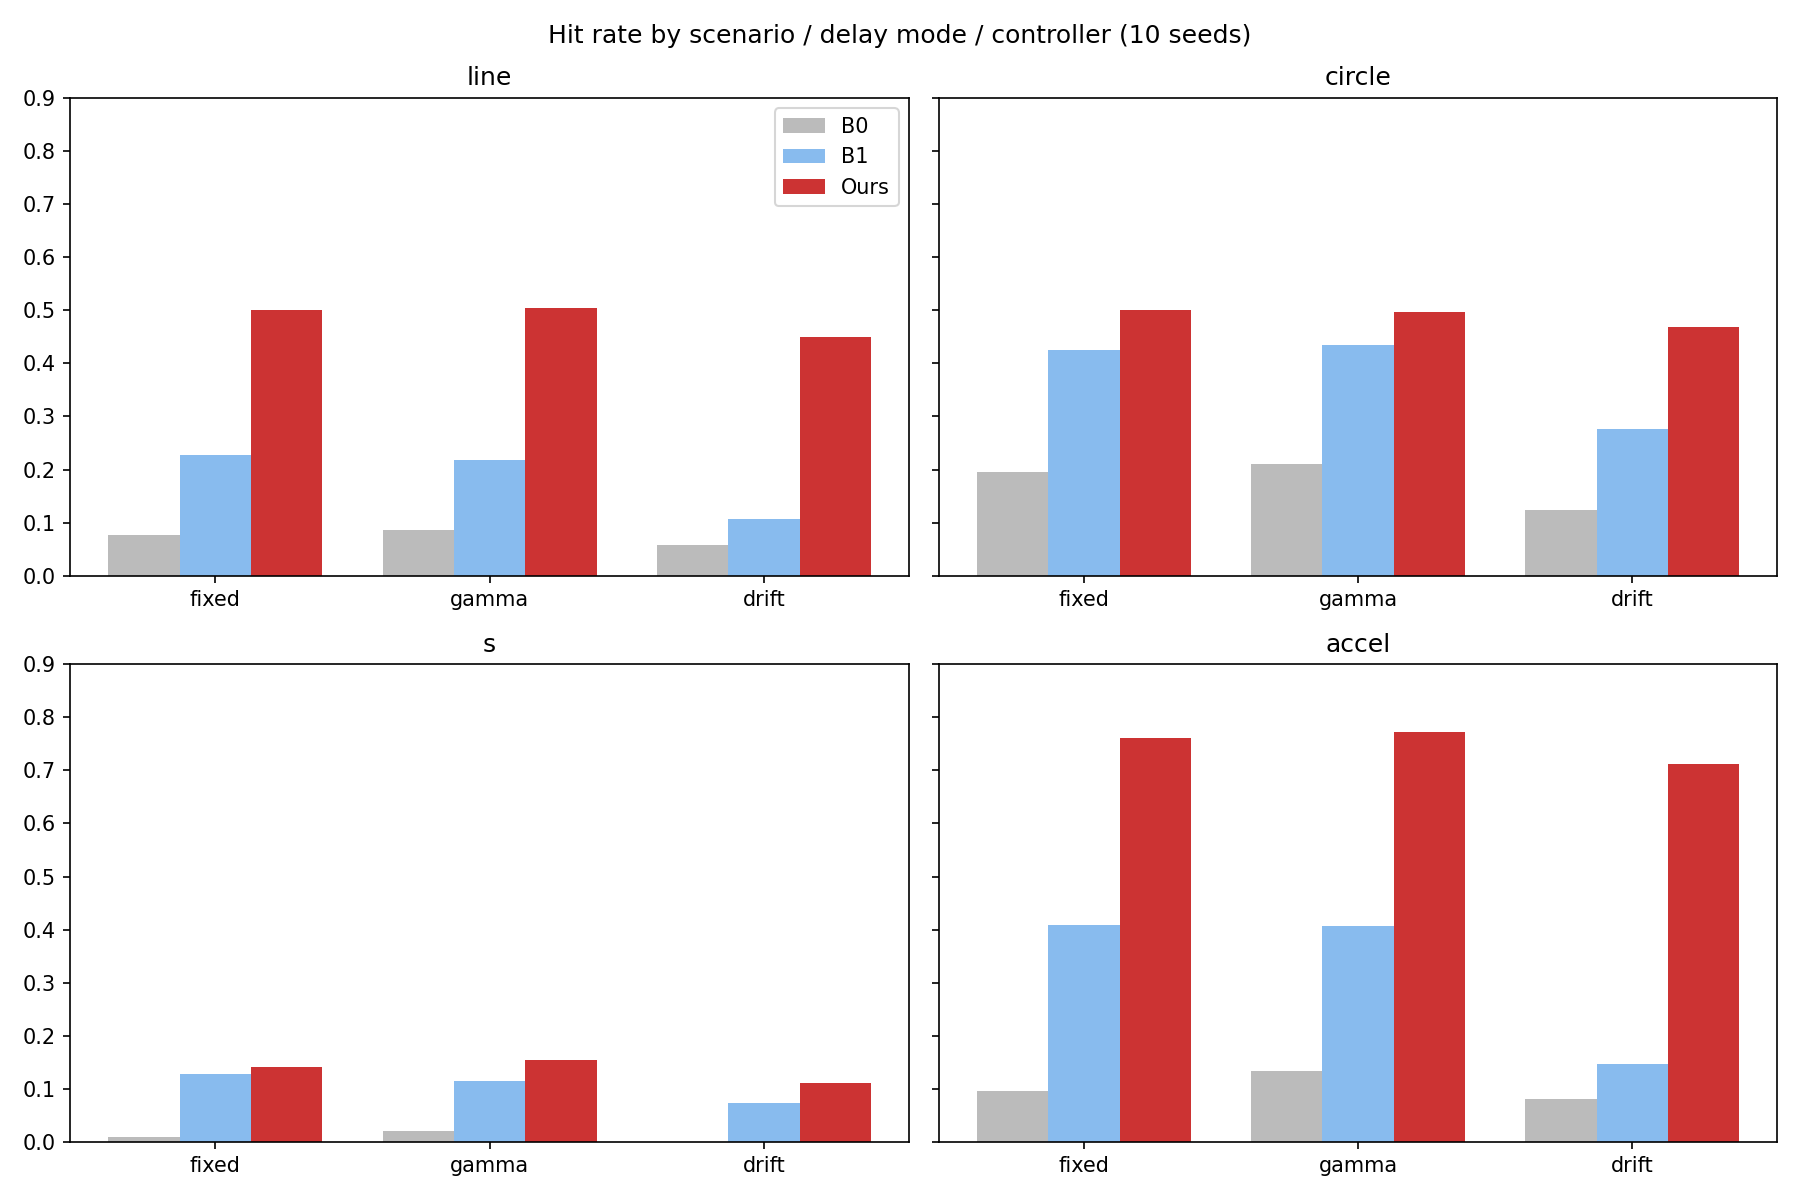
\includegraphics[width=0.9\columnwidth]{results_hitrate.png}
\caption{Hit rate by scenario / delay mode / controller (10 seeds).}\label{fig:hit}
\end{figure}
\begin{figure}[t]\centering
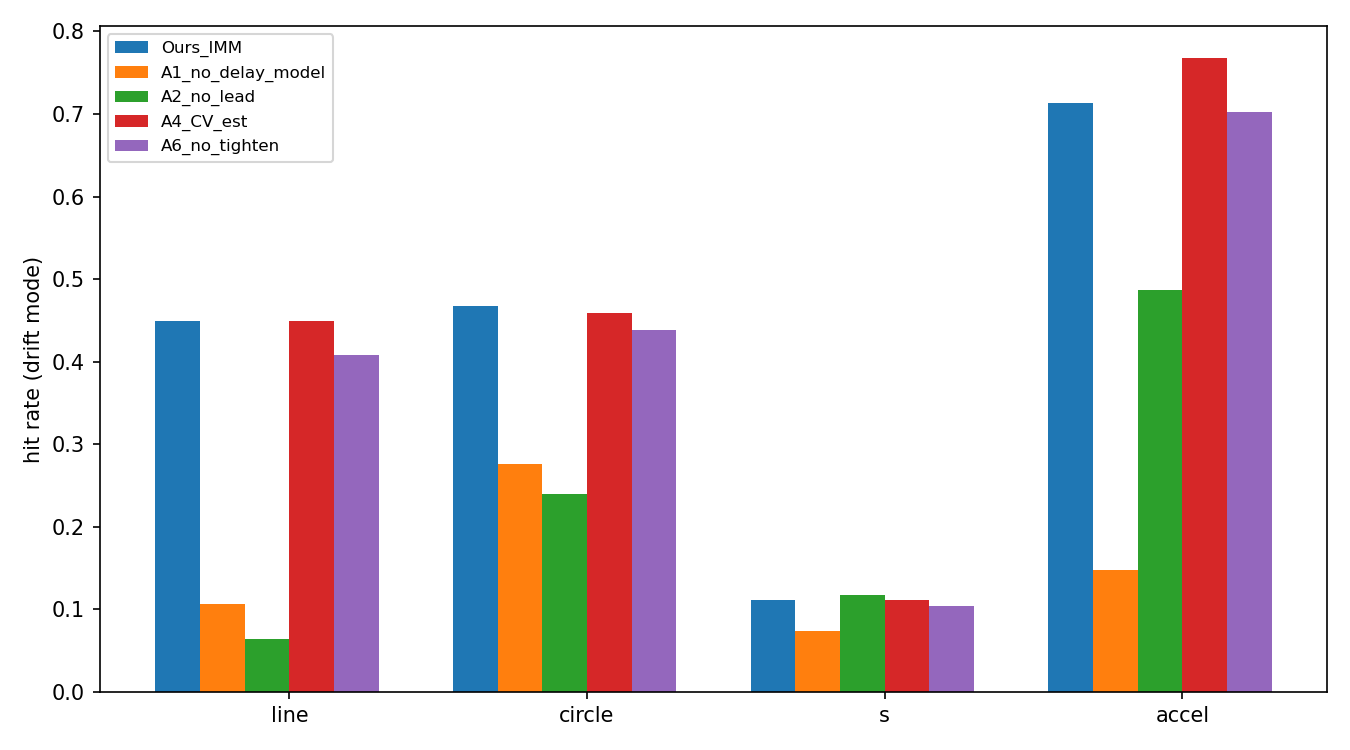
\includegraphics[width=0.9\columnwidth]{results_ablations.png}
\caption{Ablations under the drift profile.}\label{fig:abl}
\end{figure}
\section*{Data Availability}
Code, per-seed results, real-time benchmark, and latency-profiling tooling are available at \url{<repo-url>}.
\end{document}
